\chapter{Projekt aplikacji}
Aplikacja zbudowana jest w środowisku Docker\cite{docker} i składa się z czterech kontenerów w 
architekturze trójwarstwowej, uzupełnionej o oddzielny serwis NLP (ang. Natural Language
Processing) odpowiadający za działanie modelu uczenia maszynowego. Wydzielenie serwisu NLP z 
warstwy serwisowej podyktowane jest względami ekonomicznymi: lekkie serwisy wymagające
ciągłej dostępności mogą być uruchamiane na tanich, małych maszynach, natomiast serwis wykonujący 
kosztowną inferencję potencjalnie wymagający karty graficznej może być wdrożony
osobno, na wydajniejszym sprzęcie uruchamianym wyłącznie na potrzeby przetwarzania nowych książek.
\begin{figure}[htbp]
    \center
    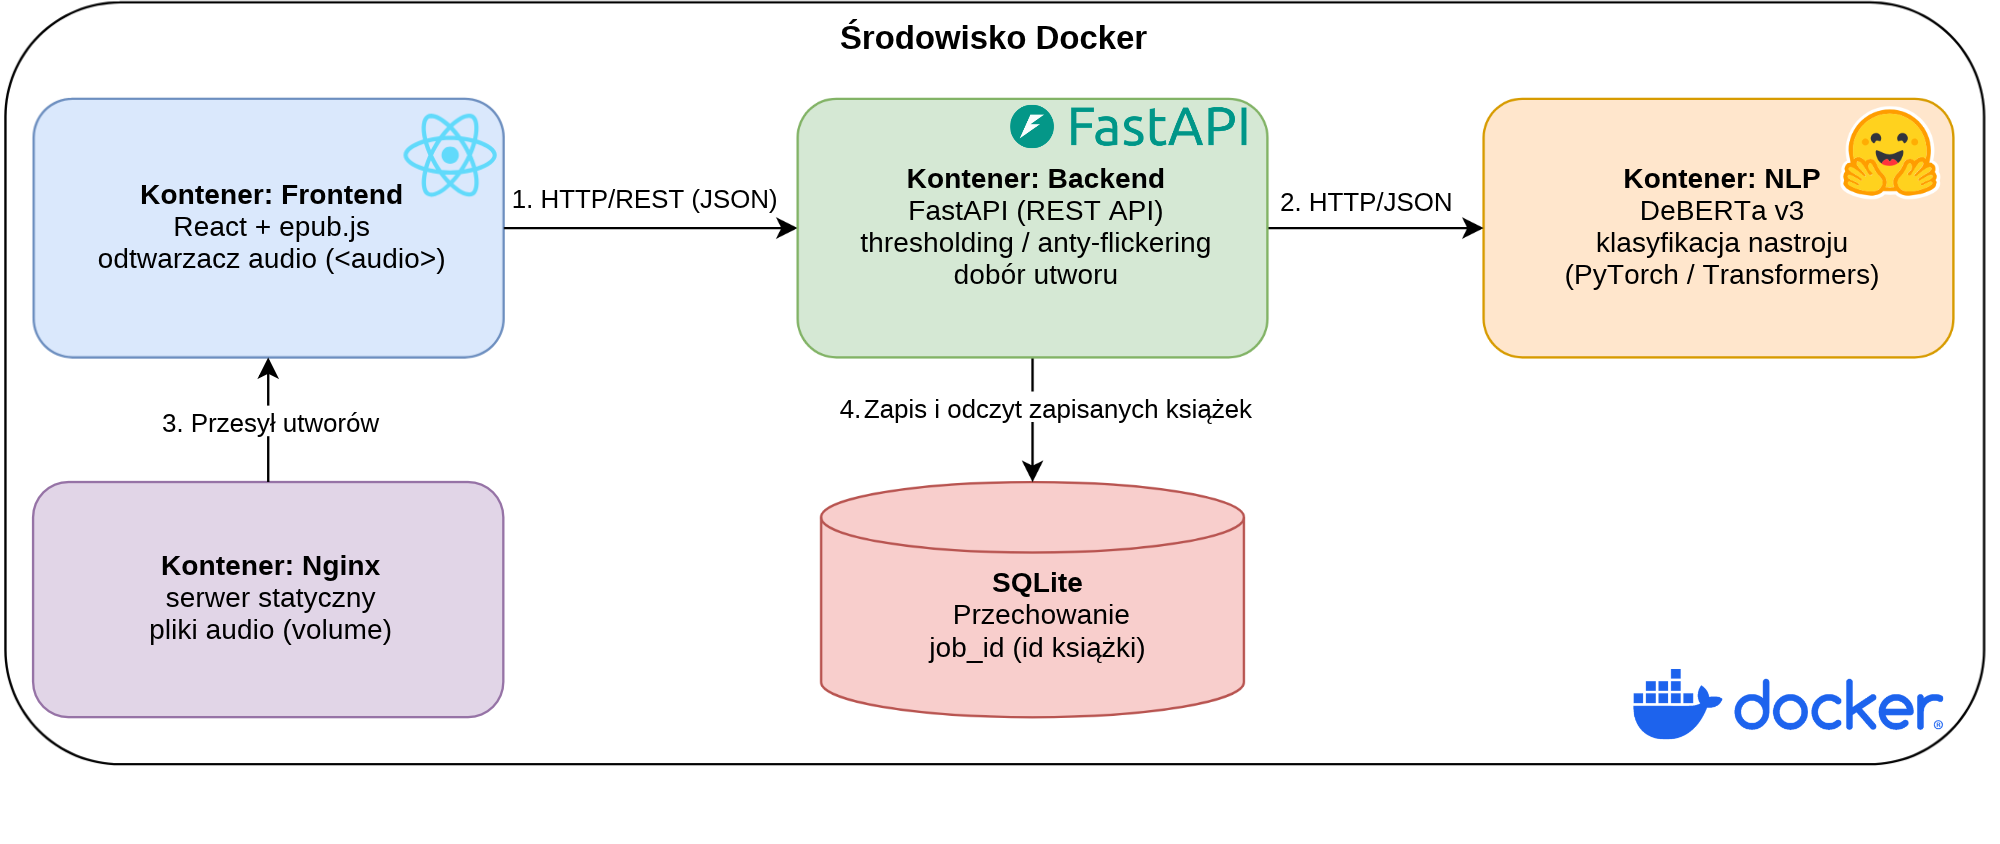
\includegraphics[width=0.9\linewidth]{figures/6/implementacja.png}
    \caption{Diagram implementacji aplikacji}
    \label{fig:app_implementation}
\end{figure}



\section{Warstwa prezentacji (Front-end)}
Warstwa prezentacji zbudowana jest przy użyciu biblioteki React\cite{React} z językiem TypeScript.
Do budowania i~pakowania aplikacji wykorzystano narzędzie Vite\cite{Vite}, które umożliwia 
parametryzację procesu budowania za pomocą zmiennych środowiskowych --- adres serwera API oraz 
serwera muzycznego przekazywane są do aplikacji w~czasie budowania obrazu Docker jako argumenty 
\textit{VITE\_API\_URL}, \textit{VITE\_MUSIC\_ORIGIN} oraz \textit{VITE\_MANIFEST}.
Gotowa aplikacja serwowana jest przez wbudowany serwer Nginx jako zestaw statycznych plików.

\subsection{Struktura komponentów}
\begin{table}[htbp]
    \centering
    \caption{Główne komponenty warstwy prezentacji}
    \label{tab:frontend_components}
    \begin{tabular}{l p{9cm}}
        \toprule
        Komponent & Rola \\
        \midrule
        App.tsx            & Główny komponent aplikacji; zarządza stanem sesji 
                                        użytkownika oraz przekazuje dane między czytnikiem 
                                        a odtwarzaczem muzycznym. \\
        file\_upload.tsx    & Formularz wgrywania pliku \textit{.epub}; 
                                        wywołuje endpoint \textit{/books/upload\_epub} 
                                        i~inicjuje proces przetwarzania. \\
        book\_reader.tsx    & Czytnik książki; odpowiada za dynamiczne 
                                        stronicowanie treści oraz raportowanie 
                                        identyfikatorów aktualnie widocznych zdań. \\
        music\_player.tsx   & Silnik odtwarzacza audio; obsługuje crossfade, 
                                        histerezę zmiany nastroju oraz dobór 
                                        utworów z~manifestu. \\
        use\_job\_polling.tsx & Hook cyklicznie sprawdzający status 
                                        przetwarzania książki; zatrzymuje polling 
                                        po osiągnięciu statusu \textit{done}. \\
        \bottomrule
    \end{tabular}
\end{table}

\FloatBarrier
\subsection{Przepływ danych między czytnikiem a odtwarzaczem}
Komunikacja między komponentem czytnika a odtwarzaczem muzycznym odbywa się 
za pośrednictwem komponentu nadrzędnego \textit{App}. Czytnik przekazuje 
w~górę poprzez wywołanie zwrotne \textit{onVisibleSentences} listę 
identyfikatorów zdań aktualnie widocznej strony wraz z~dwoma kolejnymi 
stronami (bufor \textit{lookahead}). Komponent \textit{App} przesyła te 
identyfikatory do backendu wywołując endpoint 
\textit{POST~\allowbreak/predictions/\{job\_id\}}, a~otrzymaną odpowiedź 
 zawierającą etykietę nastroju, pewność klasyfikacji oraz margines 
przewagi przekazuje do odtwarzacza jako właściwość \textit{prediction}. 
Dzięki takiemu podziałowi czytnik i~odtwarzacz pozostają od siebie niezależne 
i~nie komunikują się bezpośrednio.

\subsection{Mechanizm \textit{pollingu}}
Monitorowanie stanu przetwarzania wgranych książek realizowane jest przez 
hook \textit{useJobPolling}. Po wykryciu co najmniej jednej książki 
w~stanie aktywnym (\textit{sent}, \textit{parsing} lub \textit{predicting}) 
hook uruchamia cykliczne odpytywanie endpointu 
\textit{GET~\allowbreak/books/\{job\_id\}/status} dla każdej z~nich 
równolegle. Mechanizm stosuje wykładnicze wydłużanie interwału 
(\textit{exponential backoff}) początkowy odstęp wynosi 1~sekundę 
i~jest mnożony przez współczynnik~1,5 po każdym cyklu, aż do osiągnięcia 
maksymalnego interwału 5~sekund. Polling zatrzymuje się automatycznie 
w~momencie, gdy żadna z~książek nie pozostaje w~stanie aktywnym, 
czyli gdy wszystkie osiągnęły status \textit{done} lub \textit{error}. 
Każde żądanie opatrzone jest sygnałem \textit{AbortController}, 
co gwarantuje anulowanie trwających połączeń przy odmontowaniu komponentu 
i~zapobiega aktualizacji stanu po zniszczeniu drzewa React.

\subsection{Zarządzanie sesją}
Identyfikacja użytkownika w~systemie opiera się na mechanizmie sesji 
anonimowej, bez konieczności rejestracji ani logowania. Przy pierwszym 
uruchomieniu aplikacja wywołuje endpoint \textit{POST~\allowbreak/session/init}, 
w~odpowiedzi na który serwer generuje kryptograficznie bezpieczny token 
sesyjny i~ustawia go jako ciasteczko \textit{sid} z~flagami 
\textit{HttpOnly} oraz \textit{SameSite=Lax} na okres 30~dni. 
Wszystkie kolejne żądania HTTP wysyłane są z~opcją 
\textit{credentials:~"include"}, co powoduje automatyczne dołączanie 
ciasteczka przez przeglądarkę. Na podstawie wartości \textit{sid} backend 
przypisuje książki do konkretnej sesji przeglądarki, zapewniając izolację 
bibliotek między różnymi użytkownikami bez konieczności prowadzenia 
kont użytkowników.



\section{Warstwa serwisowa (Back-end)}
\subsection{Przetwarzanie wgranego pliku}
Przetwarzanie książki odbywa się asynchronicznie i składa się z kilku etapów.
Po wgraniu pliku w formacie \textit{.epub} warstwa serwisowa tworzy zadanie
o unikalnym identyfikatorze \textit{job\_id}, nadaje mu status \textit{queued}
i uruchamia właściwe przetwarzanie w tle. Plik jest następnie przetwarzany
przez autorską bibliotekę \textit{book-parser} (status \textit{parsing}),
a jej wynik zapisywany jest w katalogu zadania jako \textit{book.json}.
Zawartość tego pliku jest przekazywana do mikroserwisu \textit{NLP}
(status \textit{predicting}), który dla poszczególnych zdań wyznacza wartości
wymiarów VAD. Odebrane wyniki zapisywane są jako \textit{vad.json}, a zadanie
otrzymuje status \textit{done}. Błąd parsowania lub błąd komunikacji z
mikroserwisem (w tym przekroczenie czasu odpowiedzi) kończy proces ze statusem
\textit{failed}. Cykl życia zadania przedstawia rysunek~\ref{fig:book_states}.

\begin{figure}[htbp]
    \center
    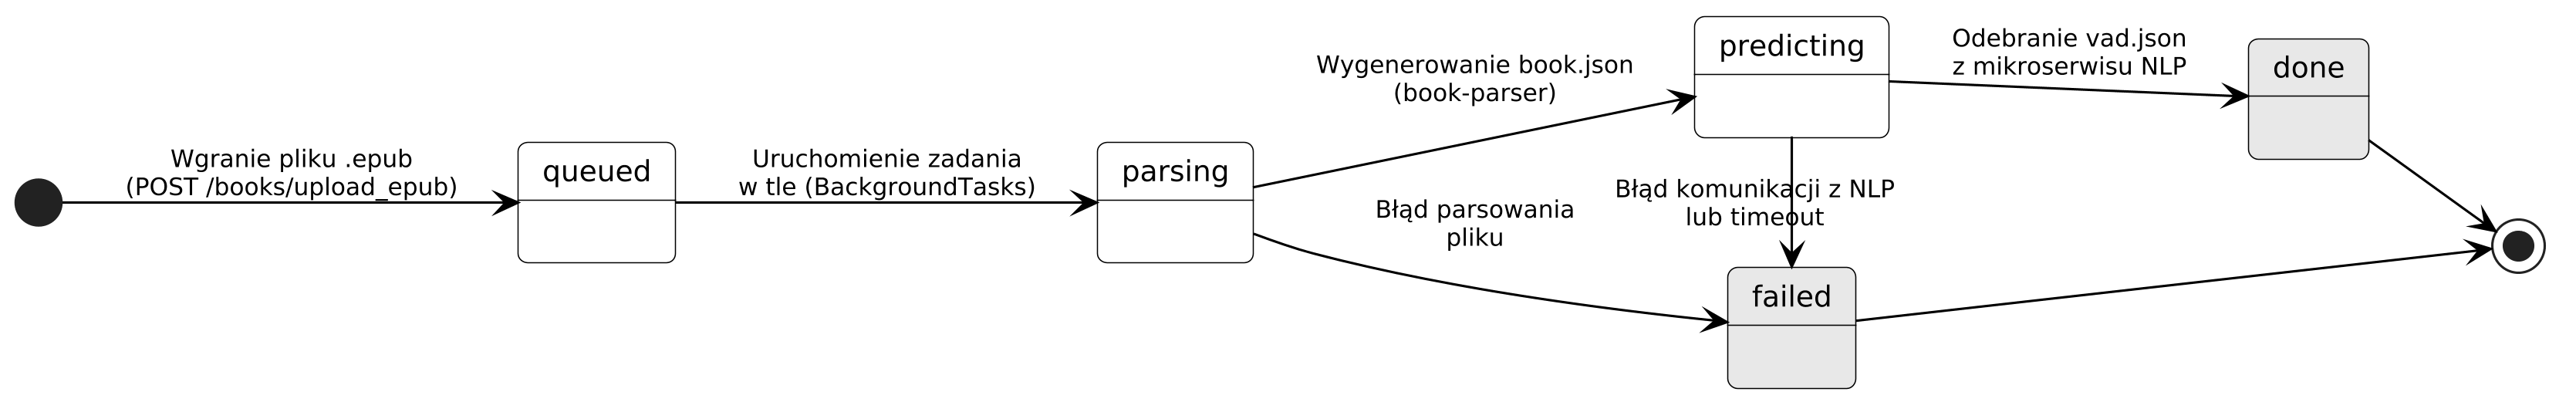
\includegraphics[width=\linewidth]{figures/6/component_diagram.png}
    \caption{Diagram stanów dla procesowania książki}
    \label{fig:book_states}
\end{figure}

\subsection{Automatyczne czyszczenie danych i retencja}
Ze względu na brak tradycyjnego systemu kont użytkowników i~oparcie identyfikacji 
wyłącznie na anonimowych sesjach przeglądarki, system wymaga mechanizmu 
zapobiegającego niekontrolowanemu zapełnianiu przestrzeni dyskowej przez 
porzucone pliki. 

W~tym celu w~modelu danych \textit{Book} zaimplementowano indeksowane pole 
\textit{last\_seen}, przechowujące znacznik czasu ostatniej aktywności powiązanej 
z~daną pozycją. Każde pobranie listy książek użytkownika (\textit{GET /books/mine}) 
aktualizuje tę wartość do bieżącego czasu UTC.

Zarządzanie retencją danych realizowane jest przez asynchroniczne zadanie 
w~tle (\textit{periodic\_cleanup}), uruchamiane w~ramach cyklu życia serwera 
(\textit{lifespan}) w~bibliotece FastAPI. Zadanie to wykonuje się cyklicznie 
co godzinę i~identyfikuje w~bazie SQLite pozycje, dla których czas od ostatniej 
aktywności przekracza ustalony okres retencji (domyślnie 3~dni). Proces czyszczenia 
przebiega dwuetapowo:
\begin{enumerate}
    \item z~systemu plików usuwany jest cały katalog roboczy powiązany 
    z~identyfikatorem \textit{job\_id} (wraz z~oryginalnym plikiem \textit{.epub}, 
    przetworzonym \textit{book.json} oraz plikiem wektorów \textit{vad.json}),
    \item rekord reprezentujący książkę zostaje trwale usunięty z~bazy danych 
    w~ramach transakcji.
\end{enumerate}
Mechanizm ten gwarantuje spełnienie wymagania niefunkcjonalnego dotyczącego 
zarządzania pamięcią masową bez ingerencji administratora systemu.


\section{Moduł przetwarzania języka naturalnego i klasyfikacji emocjonalnej}
Moduł przetwarzania \textit{NLP} stanowi niezależny mikroserwis zrealizowany 
w~ramach frameworka FastAPI, udostępniający dedykowany punkt końcowy na 
potrzeby warstwy serwisowej. Usługa przyjmuje plik \textit{book.json} 
o~strukturze przedstawionej na listingu~\ref{lst:json_processed}, zawierający 
sparsowane rozdziały i~zdania książki.

W~pierwszym etapie załadowany do pamięci model DeBERTa-v3 dokonuje wsadowej 
inferencji (\textit{batch inference}), wyznaczając ciągłe wektory w~trójwymiarowej 
przestrzeni nastroju VAD (Valence, Arousal, Dominance) dla każdego zdania 
w~tekście. 

Następnie moduł adaptuje przestrzeń emocjonalną do specyfiki analizowanej 
książki. Wartości referencyjne czterech podstawowych kategorii emocji pobrano 
ze słownika \textit{NRC VAD Lexicon}\cite{VDA-leksykon} (tabela~\ref{tab:emotion_table}). 
Na podstawie mediany oraz rozstępu percentylowego predykcji dla całej książki 
wyznaczany jest środek układu oraz współczynnik skalowania, za pomocą których 
bazowe wektory leksykonu są transformowane w~dynamiczne centroidy nastroju.

\begin{table}[htbp]
    \centering
    \caption{Wartości referencyjne centroidów emocji w modelu VAD}
    \label{tab:emotion_table}
    \begin{tabular}{l l r r r}
        \toprule
        Nazwa & Tłumaczenie & V & A & D \\
        \midrule
        JOY     & radość   &  0{,}960 &  0{,}684 &  0{,}588 \\
        SADNESS & smutek   & -0{,}896 & -0{,}424 & -0{,}672 \\
        TENSE   & napięcie & -0{,}392 &  0{,}620 &  0{,}058 \\
        CALM    & spokój   &  0{,}750 & -0{,}900 & -0{,}373 \\
        \bottomrule
    \end{tabular}
\end{table}

W~celu eliminacji fałszywych klasyfikacji w~fragmentach o~umiarkowanym ładunku 
emocjonalnym wprowadzono dodatkową klasę neutralną (\textit{NEUTRAL}). Jest ona 
definiowana jako strefa wokół wyznaczonego środka rozkładu, ograniczona promieniem 
neutralności równym 25.~percentylowi odległości euklidesowych zdań na płaszczyźnie 
Valence--Arousal. Rozwiązanie to wprowadza histerezę klasyfikacyjną, zapobiegając 
niepożądanym, zbyt częstym zmianom odtwarzanej muzyki. 

Końcowy rezultat przetwarzania zawierający wektory VAD wszystkich zdań 
oraz obliczone współczynniki adaptacyjne zwracany jest do backendu 
w~pliku \textit{vad.json}.
\begin{figure}[htbp]
    \center
    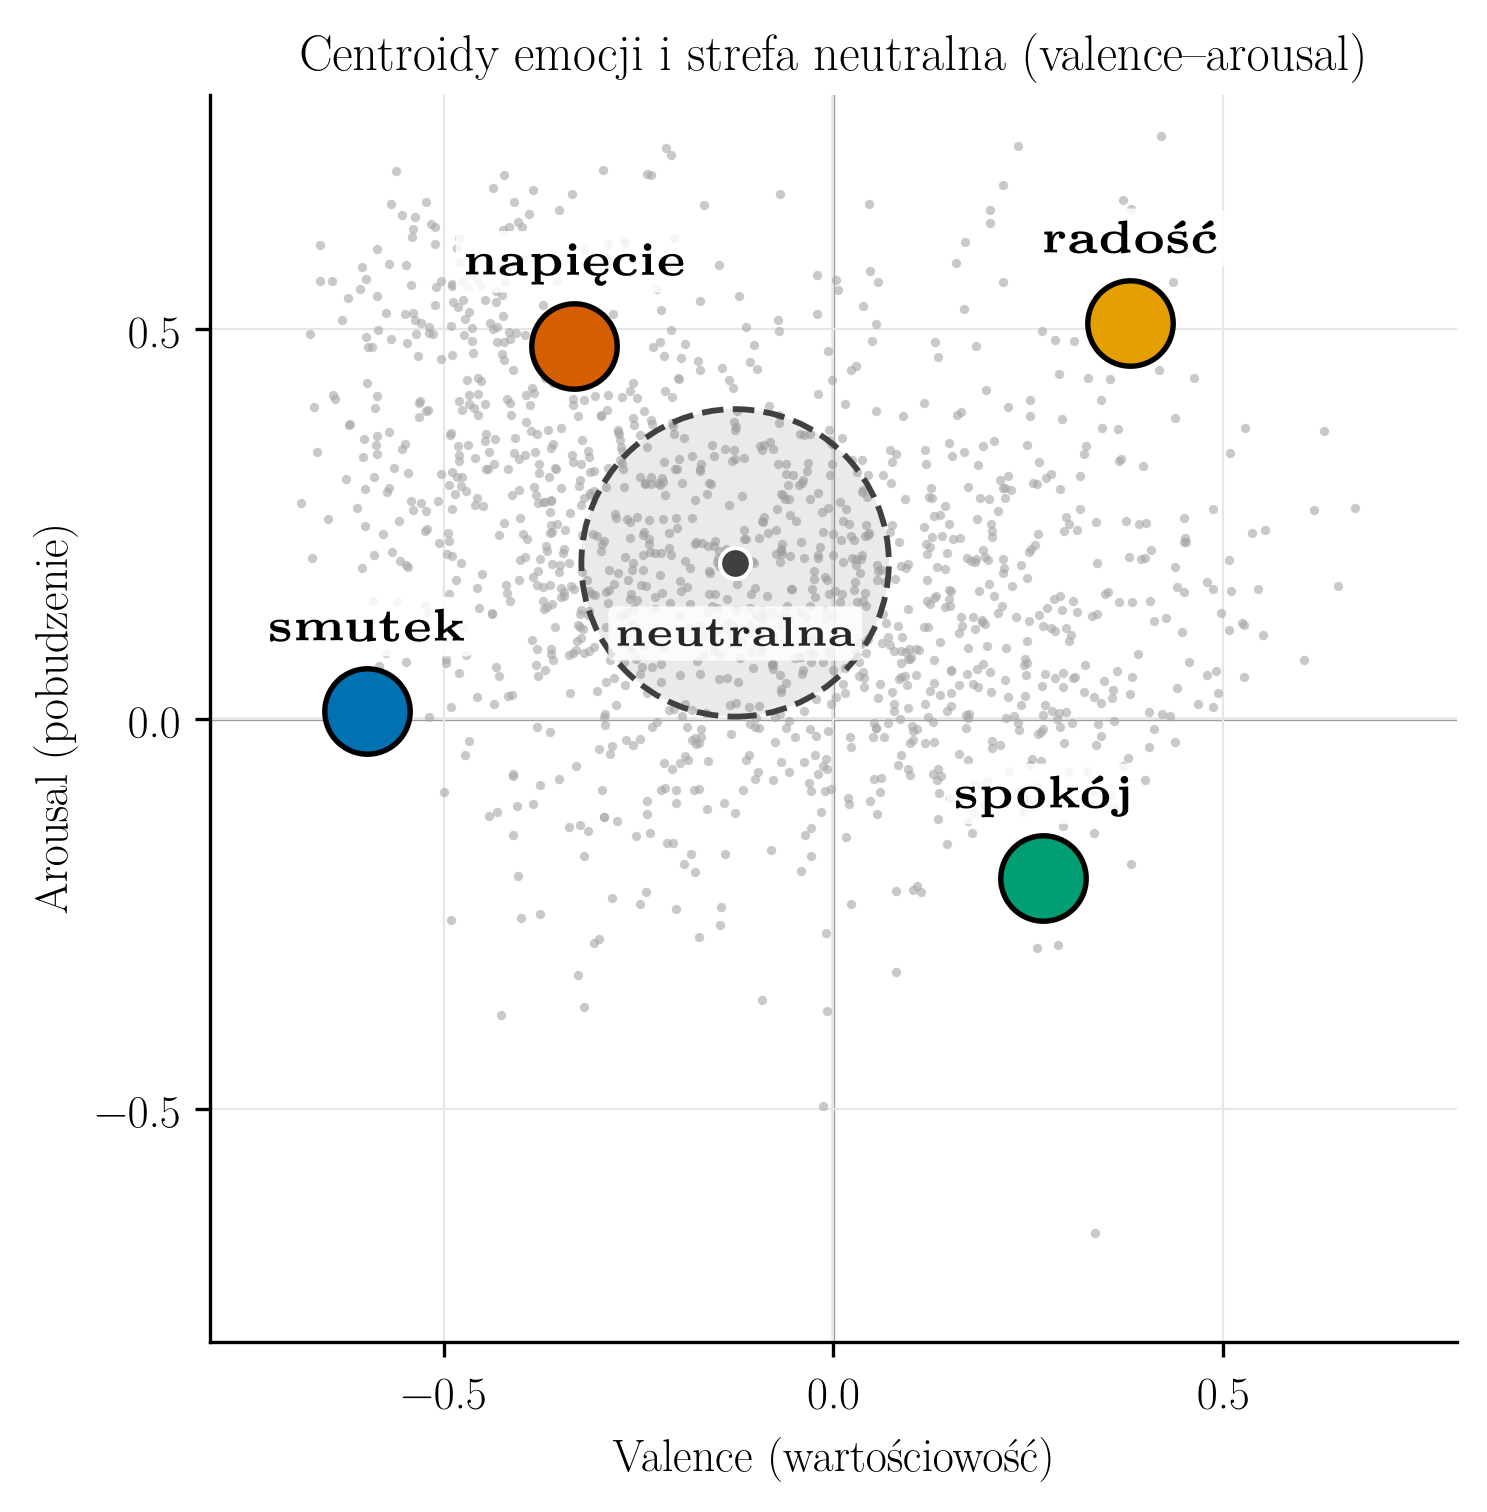
\includegraphics[width=0.7\linewidth]{figures/6/va_scatter.png}
    \caption{Przykład rozkładu przeprocesowanego pliku, zaznaczone centroidy i strefa neutralna,
    dla książki \textit{"At the mountains of madness"} H. P. Lovecraft'a}
    \label{fig:centroids}
\end{figure}
\FloatBarrier
W podanym przykładzie znaczna część predykcji skupia się wokół napięcia, ponieważ analizowany
fragment pochodzi z utworu z gatunku horroru.

\section{Środowisko uruchomieniowe i konteneryzacja}
W celu zapewnienia powtarzalności środowiska wykonawczego oraz łatwości
wdrożenia, system został w całości skonteneryzowany przy użyciu platformy
Docker\cite{docker} oraz narzędzia Docker Compose. Całość podzielono na
cztery współpracujące ze sobą usługi: interfejs użytkownika
(\textit{frontend}), serwer aplikacyjny (\textit{backend}), moduł uczenia
maszynowego (\textit{nlp}) oraz serwer plików statycznych i
strumieniowania audio (\textit{nginx}).

\subsection{Optymalizacja i budowa obrazów kontenerów}
Do budowy każdego komponentu przygotowano dedykowane pliki
\textit{Dockerfile}, stosując szereg optymalizacji:
\begin{itemize}
    \item \textbf{Wielofazowe budowanie front-endu (ang.
    \textit{multi-stage build}):} W pierwszej fazie, bazującej na obrazie
    \textit{node:22-alpine}, aplikacja kliencka jest kompilowana przy
    pomocy narzędzia Vite z wstrzyknięciem zmiennych środowiskowych
    konfigurujących adresy API. W fazie końcowej wykorzystano
    zoptymalizowany obraz \textit{nginx:alpine}, do którego kopiowany
    jest wyłącznie wynikowy katalog \textit{dist}. Eliminuje to
    konieczność instalacji środowiska Node.js na serwerze produkcyjnym i
    radykalnie zmniejsza rozmiar obrazu.
    \item \textbf{Minimalizacja zależności modułu NLP:} W kontenerze 
    przetwarzania języka naturalnego wykorzystano obraz bazowy 
    \textit{python:3.12-slim} oraz bibliotekę PyTorch w dedykowanej
    wersji procesorowej (CPU-only), eliminując narzut bibliotek CUDA
    sięgający kilku gigabajtów. Dodatkowo, wagi wytrenowanego modelu nie
    są wbudowywane w warstwy obrazu, lecz podmontowywane w trybie tylko
    do odczytu (\textit{read-only}), co pozwala na ich niezależne
    wersjonowanie.
    \item \textbf{Bezpieczeństwo warstwy backendowej:} Kontener logiki 
    biznesowej realizuje zasadę najmniejszych uprawnień poprzez
    utworzenie dedykowanego użytkownika nieuprzywilejowanego
    (\textit{appuser}), pod którego kontrolą uruchamiany jest serwer
    Uvicorn.
    \item \textbf{Automatyzacja serwera multimediów:} Kontener Nginx
    serwujący pliki muzyczne wyposażono w skrypt inicjalizacyjny
    \textit{make\_manifest.sh}, który podczas startu dynamicznie
    indeksuje katalog utworów audio i generuje plik manifestu w formacie
    JSONL.
\end{itemize}

\subsection{Silnik odtwarzania i miksowania audio}
Kluczowym elementem warstwy prezentacji jest silnik odtwarzacza audio zaimplementowany w~ramach dedykowanego hooka \textit{useMusicEngine} (komponent \textit{music\_player.tsx}). Jego
zadaniem jest dynamiczne zarządzanie ścieżkami dźwiękowymi, realizacja płynnych przejść tonalnych oraz eliminacja zjawiska gwałtownych skoków nastroju w~trakcie lektury.

\subsubsection{Histereza i tłumienie oscylacji nastroju}
Bezpośrednia zmiana podkładu muzycznego przy każdej zmianie predykcji tekstu prowadziłaby do rozpraszającego „migotania” nastrojów (\textit{mood jitter}). W~celu zapewnienia
stabilności odsłuchu wprowadzono trzystopniowy mechanizm histerezy:
\begin{enumerate}
    \item \textbf{Filtrowanie progowe pewności:} Zmiana nastroju jest rozpatrywana wyłącznie wtedy, gdy pewność klasyfikacji wynosi co najmniej $40\%$ ($\text{certainty} \ge 0{,}4$),
    a~margines przewagi nad drugą najbardziej prawdopodobną klasą wynosi minimum $0{,}1$ ($\text{margin} \ge 0{,}1$).
    \item \textbf{Minimalny okres karencji (\textit{cooldown}):} Zdefiniowano sztywny minimalny interwał stabilizacji wynoszący 20 sekund pomiędzy kolejnymi zmianami nastroju.
    \item \textbf{Odroczona zmiana stanu:} Jeśli silnik otrzyma sygnał o~nowym nastroju przed upływem okresu karencji, zdarzenie nie jest odrzucane, lecz planowane w~strukturze
    \textit{setTimeout} na czas $t_{\text{wait}} = 20\,\text{s} - (t_{\text{bieżący}} - t_{\text{ostatnia\_zmiana}})$. Po upływie tego czasu zmiana dochodzi do skutku tylko wtedy, gdy
    aktualny nastrój nadal różni się od odtwarzanego.
\end{enumerate}

\subsubsection{Adaptacyjny czas trwania przejścia}
Czas trwania miksowania ($T_{\text{fade}}$) jest skalowany dynamicznie w~zależności od pewności modelu:
\begin{equation}
    T_{\text{fade}} = 8000\,\text{ms} - \min\left(1, \frac{\text{certainty} - 0{,}4}{0{,}6}\right) \cdot 6000\,\text{ms}
\end{equation}
Dla predykcji o~wysokiej jednoznaczności ($\text{certainty} = 1{,}0$) przejście następuje zdecydowanie w~czasie około 2~sekund, natomiast przy wartościach granicznych bliskich progu
($0{,}4$) crossfade jest łagodny i~wydłużony aż do 8~sekund, co maskuje niepewność klasyfikacji.

\subsubsection{Płynna ciągłość odtwarzania (\textit{track chaining})}
W~przypadku długich fragmentów książki o~jednolitym nastroju odtwarzacz zapobiega powstawaniu przerw w~dźwięku. Poprzez nasłuchiwanie zdarzenia \textit{timeupdate} silnik kontroluje
pozycję odtwarzacza i~gdy czas do zakończenia bieżącego utworu spada poniżej 4~sekund:
\begin{equation}
    t_{\text{duration}} - t_{\text{current}} \le 4\,\text{s}
\end{equation}
automatycznie inicjuje 4-sekundowe przejście do kolejnego utworu z~tej samej kategorii nastroju wylosowanego z~manifestu, zapewniając nieprzerwane tło muzyczne (\textit{gapless
playback}).


\subsection{Komunikacja sieciowa i zarządzanie danymi}
Kontenery połączone są w ramach wspólnej, wirtualnej sieci mostkowej
(\textit{bridge}), co umożliwia wzajemną komunikację po nazwach usług za
pośrednictwem wbudowanego mechanizmu DNS Dockera. Zewnętrzne porty
wystawiono wyłącznie dla aplikacji webowej (8080), głównego API (8000) 
oraz serwera plików dźwiękowych (8800). Dostęp do serwisu NLP ograniczono
wyłącznie do wnętrza sieci kontenerowej (port 8008 nie jest publikowany
na zewnątrz hosta), co podnosi poziom bezpieczeństwa architektury.

Trwałość danych zapewniono poprzez nazwany wolumen \textit{bookdata},
przechowujący wgrane publikacje i przetworzone dane analityczne
niezależnie od cyklu życia poszczególnych kontenerów. Z kolei zbiory
plików statycznych (katalog utworów oraz wagi modeli) dołączono za pomocą
montowania wiązanego (\textit{bind mounts}) z flagą \textit{ro},
zabezpieczając je przed nieautoryzowaną modyfikacją z poziomu
uruchomionych procesów.

\subsection{Interfejs użytkownika}
